\documentclass[11pt]{article}

\newcommand{\TITLE}{Chimbuko: CODAR Framework for Performance Analysis and Visualization}
\newcommand{\AUTHORS}{Kerstin Kleese Van Dam, Shinjae Yoo, Wei Xu, Line Pouchard, \\ Hubertus Van Dam, Li Tang, Meifang Lin, Abid Malik, Shantenu Jha\\ Brookhaven National Laboratory\\ \vspace{0.2in} Kevin Huck, Sameer Shende\\ University of Oregon}

% \usepackage{mathptmx} % Close to times new roman
%\usepackage{newtxtext} % Close to times new roman
% \usepackage{newtxmath} % Close to times new roman
\usepackage{enumitem} % For tighter lists
\usepackage{cutwin,pstricks}
\usepackage{tcolorbox}
\usepackage{xcolor}

% Helvetica
\renewcommand{\rmdefault}{phv}
\renewcommand{\sfdefault}{phv}

\usepackage[font={footnotesize,bf}]{caption}

\usepackage{comment}
\usepackage{epsfig,wrapfig,url}
\usepackage[hidelinks]{hyperref}
\usepackage{pdfpages}
%\usepackage{amsfonts,amsmath,amscd,amsthm}
%\usepackage[mathscr]{euscript}
% Next line gives us superscript citations
%\usepackage[superscript,biblabel]{cite}
\usepackage{caption,subcaption}

\textfloatsep = 0.1in
\usepackage{array}
\newcolumntype{L}[1]{>{\raggedright\let\newline\\\arraybackslash\hspace{0pt}}m{#1}}
\usepackage{amsmath,amssymb}



\newif\iffinal

\finaltrue

\iffinal
  \newcommand\todo[1]{}
  \newcommand\ian[1]{}
\else
  \newcommand\todo[1]{{\color{red}#1}}
  \newcommand\ian[1]{{\color{blue}[Ian: #1]}}
\fi

\setlength{\textwidth}{6.5in}
\setlength{\oddsidemargin}{0in}
\setlength{\evensidemargin}{0in}
\setlength{\textheight}{9.0in}
\setlength{\topmargin}{0in}
\setlength{\headheight}{0in}
\setlength{\headsep}{0in}
\setlength{\footskip}{.5in}
\setlength{\parskip}{.05in}
\setlength{\parindent}{0in}
\usepackage[explicit]{titlesec}

\titleformat{\section}
  {\normalfont\Large\bfseries}{\thesection}{1em}{#1}[{\titlerule[0.8pt]}]

\usepackage{titlesec}
\titlespacing{\section}{0pt}{*2}{*1.35}
\titlespacing{\subsection}{0pt}{*1.35}{*0.15}
%\titleformat{\subsection}[runin]{\bfseries}{\thesubsection}{1em}{}[.]

%\titleformat{ command }[ shape ]{ format }{ label }{ sep }{ before-code}
%\titleformat{\subsubsection}[runin]{\slshape}{\thesubsubsection}{1em}{}[.]
\titleformat{\subsubsection}[runin]{\bfseries}{\thesubsubsection}{1em}{#1}[.]
\titlespacing{\subsubsection}{0pt}{*0.105}{*1.00}

%\titleformat{\paragraph}[runin]{\bfseries}{\theparagraph}{1em}{}[.]
\titleformat{\paragraph}[runin]{\slshape}{\theparagraph}{1em}{#1}[.]
\titlespacing{\paragraph}{0pt}{*0.105}{*1.00}

\titleformat{\subparagraph}[runin]{}{\thesubparagraph}{1em}{\underline{#1}}[.]
%\titleformat{\subparagraph}[runin]{\bfseries}{\thesubparagraph}{1em}{}[.]
\titlespacing{\subparagraph}{0pt}{*0.105}{*1.00}

\setcounter{tocdepth}{2}
\setcounter{secnumdepth}{4}

\usepackage{listings} % for code listings

\newcommand\code[1]{{\tt #1}}

\lstdefinestyle{ShellStyleInLine}
{
	language=Python,
	frame=shadowbox, rulesepcolor=\color{gray},
	basicstyle = \ttfamily,
	upquote=true,
	escapechar=`,
	numbers= none,
	moredelim=[il][]{--latexlabel},
	otherkeywords={self},             % Add keywords here
	commentstyle=\color{blue},
	keywordstyle=\bfseries\color{black},
	emph={MyClass,__init__},          % Custom highlighting
	emphstyle=\bfseries\color{myred},    % Custom highlighting style
	%frame=tb,                         % Include this to remove shadows
	showstringspaces=false            %
}

\definecolor{mGreen}{rgb}{0,0.6,0}
\definecolor{mGray}{rgb}{0.5,0.5,0.5}
\definecolor{mPurple}{rgb}{0.58,0,0.82}
\definecolor{backgroundColour}{rgb}{0.95,0.95,0.92}

\lstdefinestyle{CStyle}{
    backgroundcolor=\color{backgroundColour},
    commentstyle=\color{mGreen},
    keywordstyle=\color{magenta},
    numberstyle=\tiny\color{mGray},
    stringstyle=\color{mPurple},
    basicstyle=\footnotesize,
    breakatwhitespace=false,
    breaklines=true,
    captionpos=b,
    keepspaces=true,
    numbers=left,
    numbersep=5pt,
    showspaces=false,
    showstringspaces=false,
    showtabs=false,
    tabsize=2,
    language=C
}



\begin{document}
\pagestyle{empty}

\title{\TITLE{}}
\date{}
\author{Kerstin Kleese Van Dam, Shinjae Yoo, Wei Xu, Line Pouchard, \\ Hubertus Van Dam, Li Tang, Meifang Lin, Abid Malik, Shantenu Jha\\ Brookhaven National Laboratory\\ \\ Kevin Huck, Sameer Shende\\ University of Oregon}


{\em \ }

\vspace{0.1in}

\begin{center}

{\Large \textbf{CODAR Design Document}}

\vspace{0.3in}

{\huge \textbf{\TITLE{}}}

\vspace{0.2in}

\large{Version of \today}

\end{center}

\vspace{0.2in}

\begin{center}

\AUTHORS{}

\end{center}

\vspace{2in}

\begin{center}
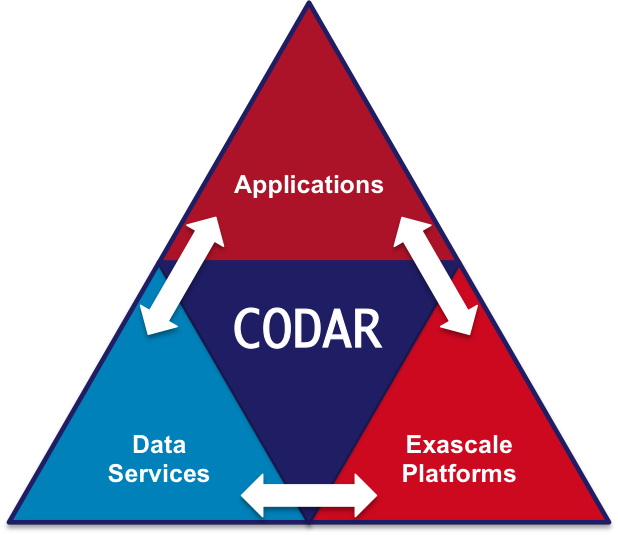
\includegraphics[width=3in]{Figs/CODAR.png}
\end{center}

\vspace{1in}




\pagebreak

\renewcommand{\contentsname}{{\huge Table of contents}}

\tableofcontents

\clearpage
\maketitle

\pagestyle{plain}
\setcounter{page}{1}

\section{Introduction}
The Chimbuko framework captures, analyzes, and visualizes performance metrics for complex scientific workflows that enables investigations into co-design tradeoffs for online data analysis and reduction on extreme-scale machines.
Chimbuko helps to compare different runs at high and low levels of metric granularity. Chimbuko provides this capability in both offline and online (in-situ) modes. Because capturing performance metrics can quickly escalate in volume and provenance can be highly verbose, Chimbuko includes a data analysis module for data reduction. 

Chimbuko enables co-design studies by allowing scientific applications and workflows to profile their execution patterns on traditional and heterogeneous architectures.  The detailed metrics and information (a.k.a. provenance of the execution) are extracted and then reduced and visualized by the Chimbuko analysis and visualization modules, thus providing insights into the behavior of the codes and workflows at scale.
%% for the purpose of code optimization and new code development.  
Using provenance, Chimbuko provides these insights for both single applications and the complex orchestrated workflows that are becoming more prevalent to organize complex code execution.

Currently, Chimbuko provides performance visualization and data analysis in an offline mode.  The next release of the framework will provide performance visualization and data analysis, helped by provenance information, for online performance analysis. Prescriptive provenance will assist in selecting features of interest in both the scientific results and the performance metrics.


\section{Stakeholders}

\subsection{ECP Applications}
Stakeholders include scientific applications that are part of the ECP program. We have consulted many and received positive feedback regarding the usefulness to them of a system such as Chimbuko. ECP applications that exhibit unexplained variability in performance, strong data reduction needs, and different types of workflows are poised to benefit from the Chimbuko technology.

\subsection{Software Technologies}					
ECP software technology  projects such as ADIOS, Cinema, Swift, SZ, and ZFP are all potential contributors of software components that may be integrated into the Chimbuko framework.

%%%% TSM:
%%%% Candle -- this is an application development project
%%%% Spack -- package manager; not clear they will provide technology to Chimbuko


\section{Use cases}
We have following use cases:

\subsection{NWCHEM}
The NWChemEx project we will study processes involving transmembrane proteins and zeolite catalysts. The processes of interest require the calculation of free energies and the dynamics of the molecular structures. In addition, to simulate realistic molecular environments, the molecular structures will have at least 100,000 atoms, different regions may be evaluated at different levels of approximation, and the simulations will work with time steps of about one femtosecond.  Hence, to sample enough of the phase space on the order of one million time steps will be evaluated. The simulation requires the evaluation and forces to update the molecular structures. While these calculations are executed, the statistics needed for the free energies are collected. In addition, selected structures along the trajectory will be stored, so that additional properties for those structure can be calculated. These additional properties will facilitate comparing the calculated trajectories against experimental observations.  Hence, the workflow will include a large number of cores calculating the energies and forces and a small number of cores analyzing the results and storing selected time steps for more detailed simulations. 

%\subsubsection{Requirements for the Online Performance Analysis}
A large number of parameters define the total amount of work performence in particular parts of the simulation and varying the amount of work will change the optimal work distribution. Performance characteristics will be recorded in a way that enables comparison against prior simulations to establish the figures of merit of the development. This requires capturing some base characteristics that are always the same. 
For specific performance optimizations, we will capture the performance of specific parts of the code, depending, for example, on the functionality of interest, on the characteristics of the data distribution, or on the granularity of the tensor blocks and associated task sizes. 
%% Dependent on these kinds of characteristics the data collection may be turned on or off. 
The shear volume of the data expected requires the analysis to be performed online.

To extract and analyze interesting events both for performance and scientific results with online analysis, prescriptive provenance will be extracted by Chimbuko.  This provenance extraction is needed to provide the execution metrics used to build training sets, classify features of interest, and select relevant events. 

\subsection{Lattie QCD}
Last year, we used TAU to benchmark a single lattice QCD calculation \url{https://github.com/meifeng/Example-LatticeQCD-With-TAU}.   This sinngle calculation is not representative of the typical production lattice QCD simulations, which are orchestrated in workflows consisting of several complex components, including propagator calculations and contractions. Provenance needs to be extracted and persisted as workflows exhibit complex interdependencies at runtime to enable diagnosis of latencies and bottlenecks. The performances of these calculations are often limited by the data transfer rates. I/O can also be a limiting factor for some algorithms in the lattice QCD workflow. This year, while the lattice QCD code is undergoing constant development, we will use Chimbuko to get a more comprehensive understanding of the performance bottlenecks both to guide our development and to provide feedback to the tool developers.
%% As the code is evolving to adapt to pre-exascale architectures such as Summit, we will target to have the first comprehensive study of the various performance metrics related to lattice QCD simulations at the beginning of FY19. 

\subsection {LAMMPS}
LAMMPS (Large Scale Atomic/Molecular Massively Parallel Simulator) is a widely used molecular dynamics simulation engine for studying materials. Our LAMMPS use case is a workflow composed of three components: (1) the LAMMPS application; (2) the Voro++ analytics engine; and (3) an ADIOS-based parallel data writer (stage\_write). The workflow is configurable, so that LAMMPS can communicate with Voro++ either directly or through stage\_write. The flexibility of the LAMMPS use case can help explore performance tradeoffs on different machines when selecting different communication strategies.

\subsection{Fusion}
Some members of the CODAR team and other ECP projects collaborated to produce an integrate demo using ECP technologies to couple two fusion simulations, one for the core of the plasma and one for the edge, each running on Titan.  ADIOS was used for data exchange at every timestep and TAU captured and aggregated performance data at runtime. The performance data measurement was limited to MPI and ADIOS events and overall application performance.  The performance data was analyzed at runtime, extracting MPI and PMI coordinate information, so that the performance data could be visualized at runtime using the PMI coordinates.  In coupling, we need to analyze aspects of the communication pattern not only between the core and edge codes but also the inter communications of each application to decide optimal placement of coupling processes.  Prescriptive provenance specifies detailed metrics of this communication. 
The performance data extraction was simplified to produce 2D scatterplots of memory consumption and FLOPS for each process to provide a ``dashboard'' for runtime observation.  This simulation could benefit from Chimbuko integration by introducing anomaly detection and richer visualization than is currently provided. 


\section{Requirements}



\begin{enumerate}[label=R-\arabic*)]
\item TAU and SOSFlow frameworks from the University of Oregon will provide the BNL team with infrastructure to make performance data accessible online ( i.e., performance monitoring) in a form that permits in situ analysis and reduction.
\item NWChem Version, Compilation, Run instruction and test case.
\item XGC Version, Compilation, Run instruction, and test case.
\item QCD Version, Compilation, Run instruction and test case. 
\item LAMMPS Version, Compilation, Run instruction and test case.
\item The Chimbuko framework should be able to run on MIRA, Titan, Theta, and more systems.
\item Information requirements from BNL to the Oregon team. See Section~\ref{subsection:features}.
\end{enumerate}


\section{Related work}

Workflows are increasingly important in orchestrating complex scientific processes in extreme scale and highly heterogeneous environments. To date, however, we cannot reliably predict, understand, and optimize workflow performance. Sources of performance variability and in particular the interdependencies of workflow design, execution environment, and system architecture are not well understood. While there is a rich portfolio of tools for performance analysis modeling and prediction for single applications in homogeneous computing environments~\cite{sonar, TAU, ScoreP, HPCToolkit}, these are not sufficient for workflows, due to the number and heterogeneity of the involved workflow and system components and their strong interdependencies. In addition, no tool currently tracks the performance of workflow components as it relates to provenance. A literature review to support these claims has been published~\cite{kerstin2015design}. 


\section{Design}
The main design components are: (1) Introspection, (2) Provenance, (3) Data Analysis and (4) Visualization. 
Figure~\ref{designfig:1} shows the interaction among the main components.

\begin{figure}[th!]
 \centering
  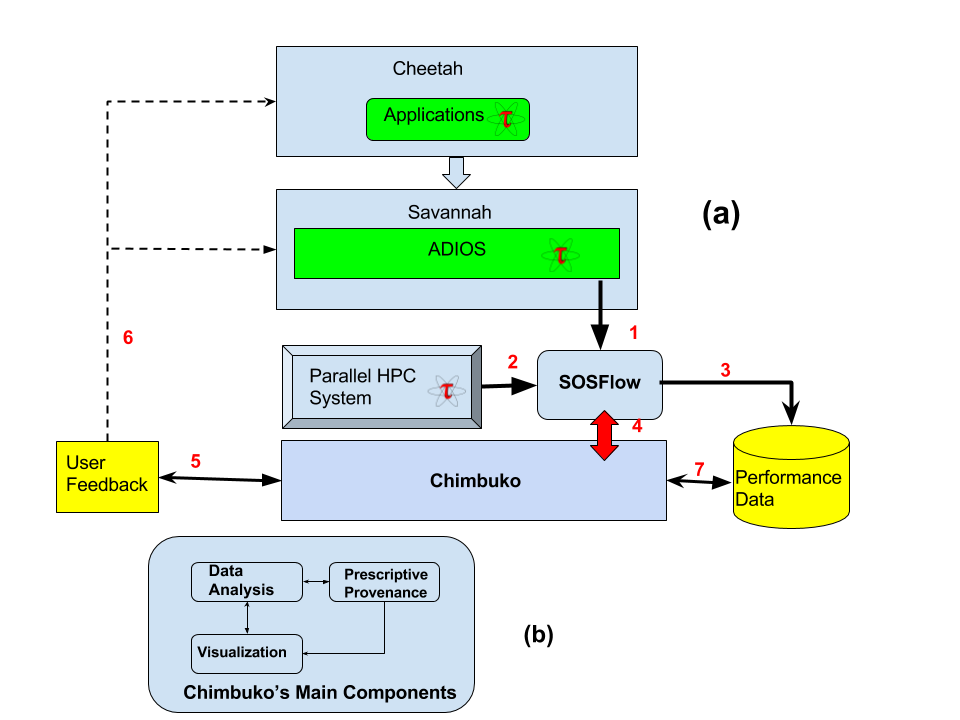
\includegraphics[width=0.65\textwidth]{Figs/Online_Chimbuko}
 \caption{(a) Introspection (b) Chimbuko's main components.}
\label{designfig:1}     
 \end{figure}

\begin{itemize}
\item {\bf{Arrow-1:}} TAU plugin extracts information from application and ADIOS for SOSFlow. 
\item {\bf{Arrow-2:}} TAU plugin extracts system information for SOSFlow.
\item {\bf{Arrow-3:}} SOSFlow stores performance information in performance database.
\item{\bf{ Arrow-4:}} SOSFlow and Chimbuko interaction.
\item {\bf{Arrow-5:}} Feedback module and Chimbuko interaction.
\item {\bf{Arrow-6:}} Feedback to Cheetah and Savannah frameworks.
\item {\bf{Arrow-7:}} Interaction between Chimbuko and performance database.
\end{itemize}

The following performance features will be collected:
\begin{enumerate}
\item For each component in a workflow:
\begin{enumerate}
\item start and end timestamp
\item call stack
\item memory allocation
\item I/O in network or disk
\item total communication time
\item effective communication time
\item effective computation time
\item idle time
\item number of synchronization points/barriers
\item communication size
\item communication between functions
\item communication between nodes
\end{enumerate}
\item For each workflow:
\begin{enumerate}
\item number of components
\item amount of communication for each pair of components
\item effective communication for each pair of components
\item communication size for each pair of components
\item aggregated number of communication calls 
\item aggregated communication execution time
\end{enumerate}
\end{enumerate}
The metadata that needs to be extracted for will vary depending on the application and the node architecture where the application components are run.
For visualization, we will also require the outlier results from the analysis module in terms of the array of call ID, MPI execution ID, or workflow ID.  
We will prioritize detailed communication, understood as MPI communication, followed by I/O.  The choice of communication as a priority for data extraction is motivated by its demonstrated impact on performance for applications such as NWChem and LAMMPS. 

\subsection{Introspection (TAU + SOSFlow)}
A performance monitoring prototype will be created to enable online access to performance data. This
will consists of two parts:
\begin{enumerate}
\item Extensible Monitoring Plugin Support: TAU will be extended to provide a plugin framework where an event stream will be exported by each MPI rank. An analysis plugin will subscribe to events such as initialization/finalization, metadata values, interval event timers, and counters.  The current hardwired SOS integration will be converted to a plugin. The SOS client plugin will monitor the data stream at runtime and provide aggregation/filtering/reduction utilities.  It will also provide a feedback path to TAU in order to increase/decrease resolution of measurement (sampling rate, callpath depth, hardware counters, etc.) if/when that capability is added to TAU.
\item Online Monitoring Access: Profile, event trace, and metadata events will be provided to the analysis through SOS~\cite{Chad}. In a coupled application/workflow scenario, SOS will regularly/periodically aggregate TAU data over the SOSFlow infrastructure.  This data will be extracted from SOS through an SOS analysis extension that will output the aggregated event stream as ADIOS streaming output.  The SOS extraction client will have the ability to filter data from one or more specific nodes, rather than just an aggregated data stream.  The ADIOS stream will be used by the trace analysis tools and anomaly detection methods.
\end{enumerate}

\subsection{Provenance}
\label{subsection:features}
We will extract, aggregate, and store provenance relevant to online performance analysis and co-design studies with the TAU/SOSFlow plugin and make this information available while the simulation is running.  As provenance can be very verbose and persisting provenance for an entire run is impractical, we will persist detailed provenance {\em only} for the anomaly events or events of interest detected by online performance analysis.  Ultimately, provenance is to be persisted in SOSFlow for a moving window prior to and posterior to an event with the additional capability to increase or decrease the verbosity of provenance (size and granularity of the moving window) selected for storage around the event.  In addition, static information describing the system, runtime configuration, and  workflow or application metadata similar to what is already extracted for offline analysis will be persisted at the on start and end of the run (static information).  This prescriptive provenance,  provenance selection and use prescribed by the results of performance data analysis, is an end product of the analysis after training sets have been built.
Specifications of the moving window of provenance prior to an outlier event will be studied for tradeoffs.  For instance, we will study if this window is defined in terms of execution time or the number of time steps.  Constraints on size and tradeoffs in the amount of details needed will be balanced with usefulness to a scientific code developer.
This prescriptive provenance approach will help reduce the information passed to the data analysis and performance visualization components.

Figure~\ref{designfig:2} explains prescriptive provenance. Suppose we detect an abnormal behavior in performance for a communication intensive workflow component. The event starts at timestamp T2 and ends at timestamp T3. To analyze this event, we need all the communication information within a certain time window at the start of the event and at the end of the event. In Figure~\ref{designfig:2}, ${\bf{X}}$ shows the time window at the start of the event till timestamp T1. The software, hardware, and system information within this time window will be correlated with the communication patterns and performance behavior of the workflow when the event occurred.

\begin{figure}[th!]
 \centering
  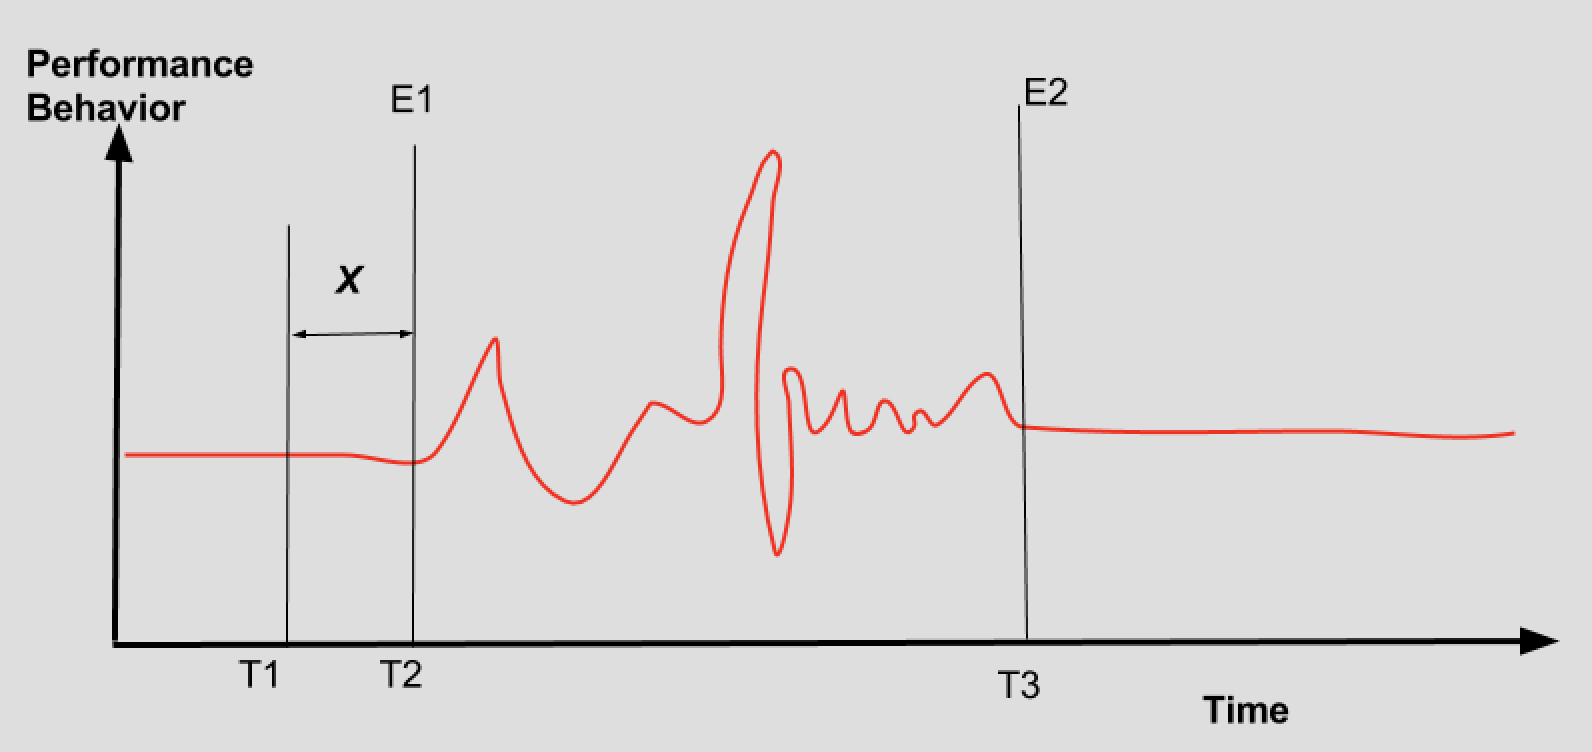
\includegraphics[width=0.5\textwidth]{Figs/Provenance}
 \caption{(a) Prescriptive Provenance.}
\label{designfig:2}     
 \end{figure}

\subsection{Data Analysis}
Last year, we prototyped offline performance anomaly detection by using a Local Outlier Factor (LOF) algorithm. This year we will implement online data analysis by designing and evaluate online anomaly detection algorithms using the features collected by SOSFlow.  The online data analysis could be implemented as two styles: (1) consumer-producer where SOSFlow will be the performance profile/trace stream producer and our online analysis will be the consumer implemented as its client; or (2) via a performance analysis plug-in within SOSFlow to obtain the performance data stream locally.

\subsection{Performance Visualization}
Last year, we developed off-line performance visualization focusing on an ``overview first, details on demand'' scheme. To enable real-time data consumption, analysis before visualization is required.  Therefore, this year, we will provide online performance visualization coupled with performance analysis.  
To establish the connection between the analysis module, SOSFlow, and the user, the visualization module will provide (1) a user exploration interface to visualize, monitor and interact with the analysis results and performance data; and (2) a back end communication channel to the analysis module and streaming data from SOSFlow.   In particular,
we will provide:
\begin{itemize}
\item A set of visual analytics modules to convey analysis results and provide interaction.
\item Methods to communicate with the data analysis module and SOSFlow. Two styles are considered: (1) passive mode, where SOSFlow or the analysis module is a server that sends update data to the visualization module as its client; and (2) active mode, where the user queries the detailed information from SOSFlow or the analysis module. 
\item Methods to maintain a local database collecting only the details of the outliers and other necessary information for users to query workflow details.
\end{itemize}


\section{Success metrics}

The online version of Chimbuko provides a runtime view of different features important to complex scientific simulation and workflows. This information to manipulate runtime configuration parameters during the execution phase to improve performance of a given workflow a new machines. Our success metrics will be the number of co-design studies and applications that can assess and visualize the performance metrics through Chimbuko.  Another success metrics is our ability to explore the performance of co-design studies by interacting with the visualization interface, which will show the outliers identified, the function call details in a call tree structure, and other information. 

\section{Work plan}

\begin{tabular}{|p{0.7in}|p{5.5in}|}\hline
\textbf{Date}  & \textbf{Milestone} \\\hline
6/31/2017 &  Demo of Chimbuko using NWCHEM and Fusion showing the initial capabilities of online analysis.\\\hline
12/31/2017 & Distribution version of Chimbuko with enhanced capabilities for online performance visualization and analysis for scientific simulation and workflow. \\\hline

\end{tabular}

\\ \\
\section{Open questions}
Open questions relevant to this work include:

\begin{itemize}
 \item What level of granularity is needed for the collected data?   The size of the data depends on the level of granularity and the level of granularity depends on the characteristics of the application.  For some applications, communication contributes significantly to latency, while for others I/O is the bottleneck. 
\item How can we scale the information collection without increasing overhead too much? Collecting a complete holistic view of the environment during runtime is important. However, if the overhead of capturing that information is too high,
then the net gain would be too small to justify online analysis. 
\item How long should we maintain the collected data?
\item Which conferences/workshops should be targeted to publish impactful papers on this work?
\end{itemize}



%\bibliographystyle{ieeetr}
%\bibliography{Bibs/z-checker.bib}
\begin{thebibliography}{1}

  \bibitem{kerstin2015design}{\em {Enabling Structured Exploration of Workflow Performance Variability in Extreme-Scale Environments}}:
  {Kleese van Dam, K., Stephan, E.G., Raju, B., Altintas, I., Elsethagen, T.O., and Krishnamoorthy, S.}, {Proc. $8^{th}$ Workshop in Many-Task Computing on Clouds, Grids, and Supercomputers (MTAGS) collocated with SC 2015}.
  
 \bibitem{Chad}{\em C. Wood et al.,: A Scalable Observation System for Introspection and In Situ Analytics-2016 5th Workshop on Extreme-Scale Programming Tools (ESPT), Salt Lake City, UT, 2016, pp. 42-49.
doi: 10.1109/ESPT.2016.010}
  
  \bibitem{sonar} {\em Lammel S., Zahn F., Fr�ning H. (2016) SONAR: Automated Communication Characterization for HPC Applications. In: Taufer M., Mohr B., Kunkel J. (eds) High Performance Computing. ISC High Performance 2016.}
  
 \bibitem{TAU} {\em S. Shende, A. D. Malony, J. Cuny, K. Lindlan, P. Beckman and S. Karmesin, Portable Profiling and Tracing for Parallel Scientific Applications using C++, Appears in: Proceedings of SPDT'98: ACM SIGMETRICS Symposium on Parallel and Distributed Tools, pp. 134-145, Aug. 1998.}
 
 \bibitem{ScoreP}{\em Kn�pfer A. et al. (2012) Score-P: A Joint Performance Measurement Run-Time Infrastructure for Periscope, Scalasca, TAU, and Vampir. In: Brunst H., M�ller M., Nagel W., Resch M. (eds) Tools for High Performance Computing 2011. }
 
 \bibitem{HPCToolkit} {\em L. Adhianto, S. Banerjee, M. Fagan, M. Krentel, G. Marin, J. Mellor-Crummey, and N. R. Tallent. HPCToolkit: Performance tools for scientific computing. In SC '08: Proc. of the 2008 ACM/IEEE Conference on Supercomputing, New York, NY, USA, 2008. ACM.}
 
\end{thebibliography}
\end{document}

